\chapter{Мультиплеты углового момента, радиальное движение и лестница осциллятора}

\section{Угловая зависимость волновой функции}

Частица в поле центральных сил имеет радиальную координату и две угловые координаты. Классически,
\begin{equation}
\mathbf L=\mathbf r\times\mathbf p
\end{equation}
сохраняется как вектор. Его направление задаёт плоскость орбиты, хотя сама орбита не обязана быть круговой.

В квантовой механике частица описывается
\begin{equation}
\Psi=\Psi(r,\theta,\phi),
\end{equation}
а угловой момент связан с зависимостью этой волновой функции от углов.

В двух измерениях есть только одна компонента углового момента — генератор вращений вокруг оси, перпендикулярной плоскости:
\begin{equation}
L_z=-i\hbar\frac{\partial}{\partial\theta}.
\end{equation}
Собственная функция с собственным значением \(\hbar\ell\) удовлетворяет
\begin{equation}
-i\hbar\frac{\partial}{\partial\theta}\psi(r,\theta)
=\hbar\ell\,\psi(r,\theta).
\end{equation}
Координата \(r\) в этом уравнении является пассивным параметром. Решение имеет вид
\begin{equation}
\psi(r,\theta)=\chi(r)e^{i\ell\theta}.
\end{equation}
Для обычной однозначной орбитальной волновой функции возвращение в ту же точку после \(\theta\to\theta+2\pi\) требует, чтобы \(\ell\) было целым числом. Радиальный множитель \(\chi(r)\) может влиять на энергию, но не влияет на это собственное значение углового момента.

Трёхмерный аналог отделяет радиальную зависимость от функций на сфере:
\begin{equation}
\Psi(r,\theta,\phi)=R(r)Y_{\ell m}(\theta,\phi).
\end{equation}
Функции \(Y_{\ell m}\) — это сферические гармоники. Их явные формулы здесь не понадобятся. Повороты действуют на угловой множитель, тогда как радиальная функция остаётся без изменения.

\section{Конечные мультиплеты углового момента}

Компоненты углового момента удовлетворяют
\begin{equation}
\begin{aligned}
[L_x,L_y]&=i\hbar L_z,\\
[L_y,L_z]&=i\hbar L_x,\\
[L_z,L_x]&=i\hbar L_y.
\end{aligned}
\end{equation}
Выберем собственные состояния \(L_z\),
\begin{equation}
L_z|\ell,m\rangle=\hbar m\,|\ell,m\rangle,
\end{equation}
и определим
\begin{equation}
L_\pm=L_x\pm iL_y.
\end{equation}
Коммутаторы
\begin{equation}
[L_z,L_\pm]=\pm\hbar L_\pm
\end{equation}
дают
\begin{align}
L_z\bigl(L_\pm|\ell,m\rangle\bigr)
&=\bigl(L_\pm L_z+[L_z,L_\pm]\bigr)|\ell,m\rangle \\
&=\hbar(m\pm1)L_\pm|\ell,m\rangle.
\end{align}
Таким образом, \(L_+\) повышает \(m\) на единицу, а \(L_-\) понижает его на единицу, если только получающийся вектор состояния не обращается в нуль.

Для конечного мультиплета существуют наивысшее и низшее состояния:
\begin{equation}
L_+|\ell,\ell\rangle=0,
\qquad
L_-|\ell,-\ell\rangle=0.
\end{equation}
Направления \(+z\) и \(-z\) связаны поворотом, поэтому конечный спектр симметричен относительно нуля. Следовательно, его значения таковы:
\begin{equation}
m=-\ell,-\ell+1,\ldots,\ell-1,\ell,
\end{equation}
а число состояний равно
\begin{equation}
2\ell+1.
\end{equation}
Поскольку соседние значения отличаются на единицу, крайние точки могут быть целыми или полуцелыми. Обычные орбитальные сферические гармоники реализуют целочисленный случай; абстрактная алгебра углового момента допускает также полуцелые мультиплеты.

\begin{classroomqa}
\lecturetimestamp{00:16:12}
\audiencequestion{Может ли мультиплет углового момента содержать бесконечно много состояний?}
\lecturerresponse{Такую возможность можно рассматривать, но здесь она не понадобится. Вообще говоря, угловой момент обычно повышает энергию, когда остальные характеристики состояния фиксированы, поэтому состояния с бесконечным угловым моментом несущественны при обсуждении состояний с конечной энергией.}
\end{classroomqa}

\section{Общее значение \texorpdfstring{\(L^2\)}{L в квадрате}}

Оператор, измеряющий квадрат модуля углового момента, равен
\begin{equation}
L^2=L_x^2+L_y^2+L_z^2.
\end{equation}
Упорядоченное произведение лестничных операторов имеет вид
\begin{align}
L_-L_+
&=(L_x-iL_y)(L_x+iL_y) \\
&=L_x^2+L_y^2+i[L_x,L_y] \\
&=L_x^2+L_y^2-\hbar L_z.
\end{align}
Следовательно,
\begin{equation}
L^2=L_z^2+\hbar L_z+L_-L_+.
\end{equation}
Применим это тождество к наивысшему состоянию. Поскольку \(L_+|\ell,\ell\rangle=0\),
\begin{align}
L^2|\ell,\ell\rangle
&=\left(L_z^2+\hbar L_z+L_-L_+\right)|\ell,\ell\rangle \\
&=\hbar^2\left(\ell^2+\ell\right)|\ell,\ell\rangle,
\end{align}
и, следовательно,
\begin{equation}
L^2|\ell,\ell\rangle
=\hbar^2\ell(\ell+1)|\ell,\ell\rangle.
\end{equation}
Квадрат модуля не равен \(\hbar^2\ell^2\). Дополнительный член является следствием некоммутативности компонент углового момента.

То же значение имеет каждое состояние в мультиплете, а не только наивысшее.

\begin{classroomqa}
\lecturetimestamp{00:26:08}
\audiencequestion{В чём именно состоит упражнение, показывающее, что остальные состояния имеют то же значение \(L^2\)?}
\lecturerresponse{Покажите, что \(L^2\) коммутирует с каждой компонентой углового момента и, следовательно, с \(L_-\). Затем переставьте \(L^2\) через \(L_-\): если наивысшее состояние имеет собственное значение \(\hbar^2\ell(\ell+1)\), то следующее ниже имеет то же собственное значение. Повторяя этот аргумент, мы переносим его по всей лестнице.}
\end{classroomqa}

Действительно,
\begin{equation}
[L^2,L_i]=0,
\qquad i=x,y,z,
\end{equation}
поэтому
\begin{equation}
[L^2,L_\pm]=0.
\end{equation}
Например,
\begin{align}
L^2\bigl(L_-|\ell,\ell\rangle\bigr)
&=L_-L^2|\ell,\ell\rangle \\
&=\hbar^2\ell(\ell+1)L_-|\ell,\ell\rangle.
\end{align}
Продолжая спускаться вниз, получаем
\begin{equation}
L^2|\ell,m\rangle
=\hbar^2\ell(\ell+1)|\ell,m\rangle
\end{equation}
для каждого \(m=-\ell,\ldots,\ell\).

Противоположный порядок даёт эквивалентную факторизацию:
\begin{align}
L_+L_-
&=(L_x+iL_y)(L_x-iL_y) \\
&=L_x^2+L_y^2-i[L_x,L_y] \\
&=L_x^2+L_y^2+\hbar L_z,
\end{align}
и, следовательно,
\begin{equation}
L^2=L_z^2-\hbar L_z+L_+L_-.
\end{equation}

\begin{classroomqa}
\lecturetimestamp{00:32:05}
\audiencequestion{Можно ли разложить \(L_x^2+L_y^2\) в противоположном порядке, используя \(L_+L_-\)?}
\lecturerresponse{Да. Знак у члена с \(L_z\) меняется на противоположный. При таком порядке примените тождество к низшему состоянию, которое уничтожается \(L_-\), а не к наивысшему. Отсюда снова получается то же собственное значение \(\hbar^2\ell(\ell+1)\).}
\end{classroomqa}

Следовательно, сферические гармоники удовлетворяют
\begin{align}
L^2Y_{\ell m}
&=\hbar^2\ell(\ell+1)Y_{\ell m}, \\
L_zY_{\ell m}
&=\hbar m\,Y_{\ell m}.
\end{align}
Для каждого орбитального значения \(\ell=0,1,2,\ldots\) имеется \(2\ell+1\) функций, помеченных \(m=-\ell,\ldots,\ell\).

Для центрального потенциала,
\begin{equation}
[H,L_i]=0.
\end{equation}
Если зафиксированы радиальное собственное состояние энергии и \(\ell\), то изменение \(m\) с помощью \(L_\pm\) не изменяет энергию. Поэтому каждое такое радиальное собственное состояние порождает магнитный мультиплет размерности \(2\ell+1\).

Ниже показана целочисленная орбитальная лестница.\footnote{Диаграмма реконструирована по эскизу мультиплета и тождествам операторов, видимым на отметке \(00{:}35{:}53\) в видеозаписи лекции.}

\begin{figure}[htbp]
\centering
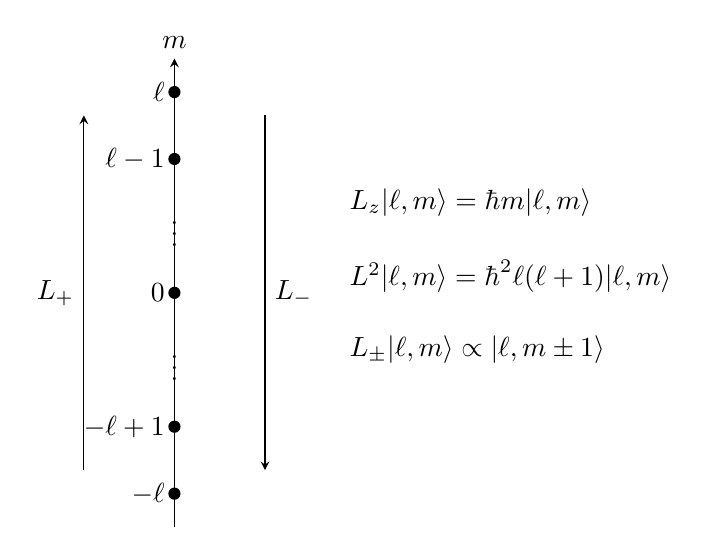
\begin{tikzpicture}[x=1cm,y=0.85cm,>=stealth]
\draw[->] (0,-3.5) -- (0,3.5) node[above] {$m$};

\fill (0,3) circle (2.2pt);
\fill (0,2) circle (2.2pt);
\fill (0,0) circle (2.2pt);
\fill (0,-2) circle (2.2pt);
\fill (0,-3) circle (2.2pt);

\node[left] at (0,3) {$\ell$};
\node[left] at (0,2) {$\ell-1$};
\node[left] at (0,0) {$0$};
\node[left] at (0,-2) {$-\ell+1$};
\node[left] at (0,-3) {$-\ell$};

\node at (0,1) {$\vdots$};
\node at (0,-1) {$\vdots$};

\draw[->] (-1.15,-2.65) -- (-1.15,2.65)
node[midway,left] {$L_+$};
\draw[->] (1.15,2.65) -- (1.15,-2.65)
node[midway,right] {$L_-$};

\node[anchor=west] at (2.1,1.35)
{$L_z|\ell,m\rangle=\hbar m|\ell,m\rangle$};
\node[anchor=west] at (2.1,0.25)
{$L^2|\ell,m\rangle=\hbar^2\ell(\ell+1)|\ell,m\rangle$};
\node[anchor=west] at (2.1,-0.85)
{$L_\pm|\ell,m\rangle\propto|\ell,m\pm1\rangle$};
\end{tikzpicture}
\caption{Целочисленный орбитальный мультиплет углового момента. \(L_+\) и \(L_-\) изменяют \(m\) на единицу, тогда как \(L^2\) остаётся равным \(\hbar^2\ell(\ell+1)\) во всём мультиплете.}
\lectureframe{00:35:53}
\end{figure}

\section{Задача о центральной силе}

Рассмотрим
\begin{equation}
H=\frac{\mathbf p^2}{2m}+V(r),
\end{equation}
где \(V\) зависит только от расстояния до начала координат. Вращательная симметрия влечёт сохранение углового момента. Классически \(\mathbf L\) имеет фиксированные модуль и направление, поэтому орбита остаётся в плоскости, перпендикулярной \(\mathbf L\). Орбита не обязана быть круговой или даже замкнутой.

Выберем координаты так, чтобы эта классическая плоскость орбиты была плоскостью \(xy\), и разложим импульс на радиальную и тангенциальную компоненты:
\begin{equation}
\mathbf p^2=p_r^2+p_\theta^2.
\end{equation}
Поскольку модуль углового момента равен
\begin{equation}
L=r p_\theta,
\end{equation}
тангенциальный вклад можно записать как
\begin{equation}
p_\theta^2=\frac{L^2}{r^2}.
\end{equation}
Гамильтониан принимает вид
\begin{equation}
H=\frac{p_r^2}{2m}+\frac{L^2}{2mr^2}+V(r).
\end{equation}
При фиксированном \(L\) это одномерная задача по радиальной координате с эффективным потенциалом
\begin{equation}
V_{\mathrm{eff}}(r)=\frac{L^2}{2mr^2}+V(r).
\end{equation}
Ниже на доске показан радиальный гамильтониан.\footnote{Исходный кадр: \texttt{\detokenize{lecture_03_frame_02.png}}, видео лекции на отметке \(00{:}47{:}15\).}

\begin{figure}[htbp]
\centering
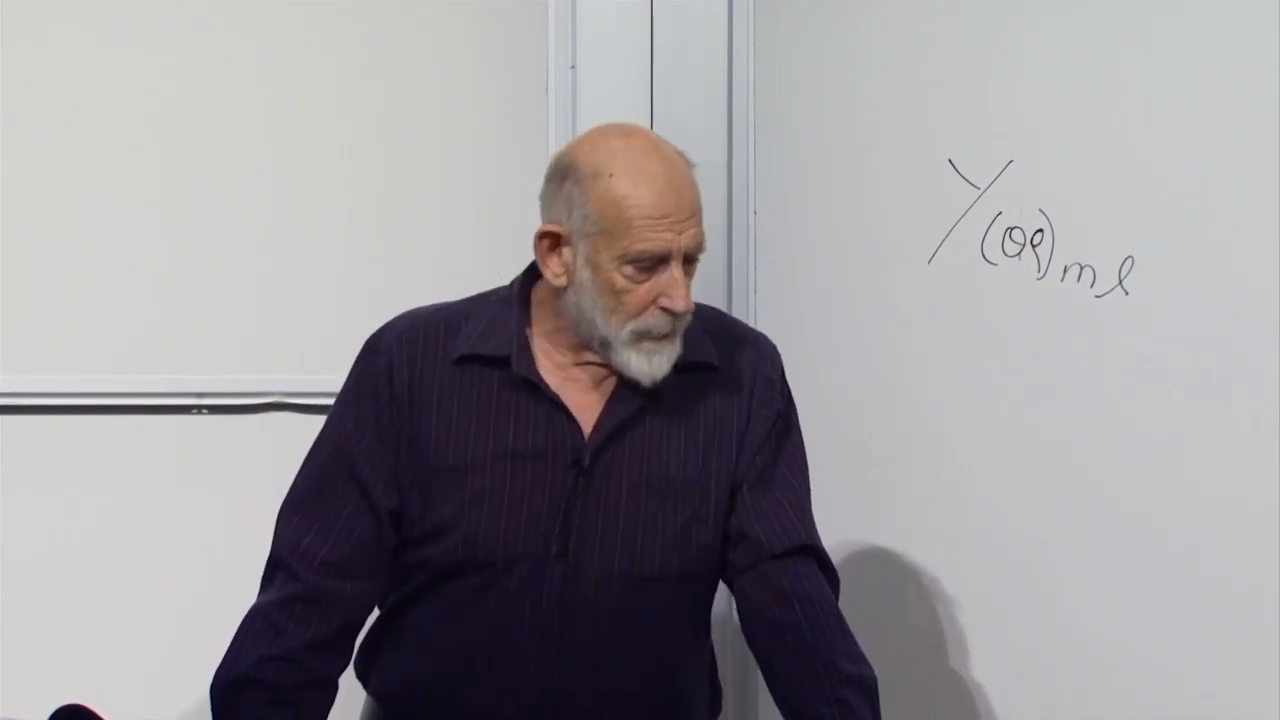
\includegraphics[width=0.9\linewidth]{lecture_03_frame_02.png}
\caption{При фиксированном классическом угловом моменте радиальный гамильтониан содержит радиальную кинетическую энергию, центробежный член \(L^2/(2mr^2)\) и центральный потенциал \(V(r)\).}
\lectureframe{00:47:15}
\end{figure}

Член \(1/r^2\) — это центробежный барьер. Он возрастает по мере приближения частицы к началу координат, поэтому соответствующая сила направлена наружу. Для обсуждаемых кулоноподобных притяжений траектория при \(L\neq0\) огибает центр вместо того, чтобы достигнуть его. При \(L=0\) барьер отсутствует.

Для притягательного кулоновского потенциала,
\begin{equation}
V(r)=-\frac{\kappa}{r},
\end{equation}
центробежный член доминирует при малых \(r\), тогда как кулоновский член убывает медленнее и доминирует при больших \(r\). При \(L\neq0\) их сумма имеет минимум. Движение в минимуме имеет постоянный радиус и потому является круговым. Связанное движение выше минимума и ниже порога убегания колеблется между наименьшим и наибольшим радиусами; в кулоновской задаче это радиальные колебания эллиптической орбиты.

\section{Редуцированное радиальное уравнение}

В квантовой механике угловая часть состояния с определённым орбитальным угловым моментом представляет собой сферическую гармонику. Запишем разделённое состояние как
\begin{equation}
\Psi_{n_r\ell m}(r,\theta,\phi)
=\frac{u_{n_r\ell}(r)}{r}\,
Y_{\ell m}(\theta,\phi).
\end{equation}
Угловой оператор \(L^2\) имеет собственное значение
\begin{equation}
L^2Y_{\ell m}
=\hbar^2\ell(\ell+1)Y_{\ell m}.
\end{equation}
Для фиксированной пары \(n_r,\ell\) будем сокращённо обозначать \(u_{n_r\ell}(r)\) через \(u(r)\). Уравнение, остающееся для редуцированной радиальной функции, имеет вид
\begin{equation}
\begin{aligned}
&-\frac{\hbar^2}{2m}\frac{d^2u}{dr^2}
+\frac{\hbar^2\ell(\ell+1)}{2mr^2}u(r)\\
&\qquad+V(r)u(r)=E_{n_r\ell}\,u(r).
\end{aligned}
\end{equation}

\editorialnote{Чисто одномерное уравнение со второй производной использует редуцированную радиальную функцию \(u=rR\). Поэтому \(\psi(r)\) в выписанном на лекции уравнении соответствует \(u(r)\), тогда как обычный радиальный множитель в \(\Psi=R(r)Y_{\ell m}\) есть \(R=u/r\). Это соглашение позволяет не рассматривать \(-i\hbar\,d/dr\) как самостоятельный эрмитов оператор радиального импульса в трёхмерном радиальном гильбертовом пространстве.}

Ниже на доске показано редуцированное радиальное уравнение.\footnote{Исходный кадр: \texttt{\detokenize{lecture_03_frame_03.png}}, видео лекции на отметке \(00{:}54{:}32\).}

\begin{figure}[htbp]
\centering
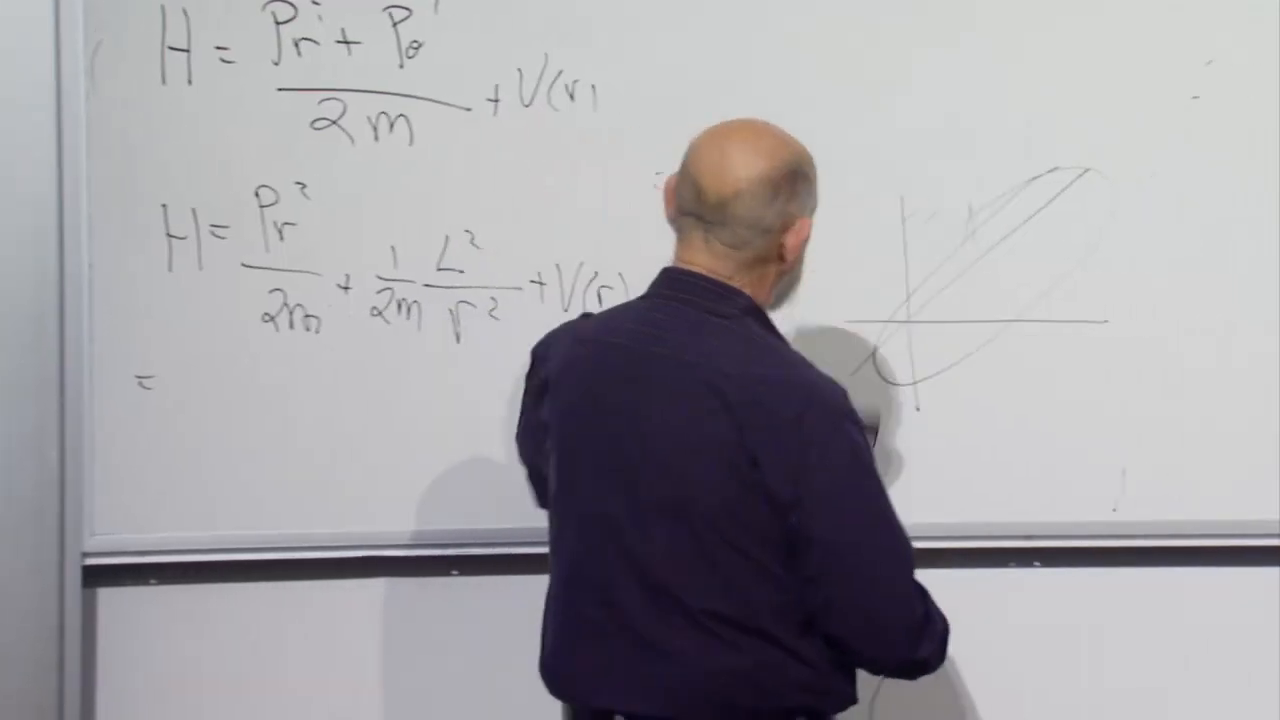
\includegraphics[width=0.9\linewidth]{lecture_03_frame_03.png}
\caption{При фиксированном \(\ell\) редуцированная радиальная волновая функция удовлетворяет одномерному уравнению Schr\"odinger с центробежным членом, пропорциональным \(\ell(\ell+1)/r^2\).}
\lectureframe{00:54:32}
\end{figure}

Трёхмерная угловая структура сведена к параметру \(\ell\). Магнитное квантовое число \(m\) не входит в радиальное уравнение.

\begin{classroomqa}
\lecturetimestamp{00:55:34}
\audiencequestion{Для данного \(\ell\) все ли \(2\ell+1\) магнитных состояний имеют одинаковую энергию?}
\lecturerresponse{Да, при условии, что радиальное собственное состояние тоже фиксировано. Для каждого выбранного \(u_{n_r\ell}\) все значения \(m=-\ell,\ldots,\ell\) имеют одинаковую энергию, потому что \(m\) не входит в радиальное уравнение. Разные радиальные собственные состояния при одном и том же \(\ell\), вообще говоря, имеют разные энергии.}
\end{classroomqa}

\begin{classroomqa}
\lecturetimestamp{00:56:03}
\audiencequestion{Почему \(L^2\) можно заменить на \(\hbar^2\ell(\ell+1)\), и как \(\ell\) связано с допустимыми значениями \(m\)?}
\lecturerresponse{Число \(\ell\) обозначает мультиплет углового момента и равно его наибольшему значению \(m\). Каждое состояние в этом мультиплете имеет одно и то же собственное значение \(L^2\), \(\hbar^2\ell(\ell+1)\), поэтому именно это собственное значение подставляется в радиальное уравнение.}
\end{classroomqa}

Явные решения через специальные функции для данного рассуждения не нужны. Важно то, как организованы решения.

\section{Радиальные узлы и энергетические уровни}

При фиксированном \(\ell\) приведённое радиальное уравнение представляет собой обычную одномерную задачу на собственные значения. Его связанные состояния упорядочены по числу внутренних узлов. Низшее радиальное состояние не имеет внутренних узлов, следующее имеет один, а следующее — два. Большее число узлов означает более быстрое изменение волновой функции; более быстрое изменение означает больший импульс и, следовательно, большую кинетическую энергию.

Каждое значение \(\ell\) задаёт свой радиальный оператор, поскольку центробежный член меняется с \(\ell\). Поэтому \(\ell=0,1,2,\ldots\) образуют отдельные радиальные башни. Положительный центробежный член сдвигает уровни вверх по мере увеличения углового момента. Каждому радиальному собственному значению при фиксированном \(\ell\) соответствует магнитный мультиплет размерности
\begin{equation}
2\ell+1.
\end{equation}
Уровни \(\ell=0\) — синглеты, уровни \(\ell=1\) — триплеты, а уровни \(\ell=2\) — квинтуплеты. Эти вырождения гарантируются вращательной симметрией; дополнительная симметрия может также сделать вырожденными состояния с разными значениями \(\ell\).

Для потенциалов атомного типа, удовлетворяющих \(V(r)\to0\) при больших \(r\), порог ухода по соглашению равен \(E=0\). Состояния с отрицательной энергией образуют дискретный связанный спектр. При \(E=0\) и выше встречается континуум рассеяния. Это утверждение зависит от поведения потенциала при больших \(r\) и не применимо к удерживающему центральному потенциалу.

\section{Особое кулоновское вырождение}

Точный нерелятивистский кулоновский потенциал обладает дополнительным совпадением уровней. Низшее радиальное состояние при \(\ell=1\) имеет ту же энергию, что и первое возбуждённое состояние при \(\ell=0\). Следующее состояние при \(\ell=1\) совпадает со вторым возбуждённым состоянием при \(\ell=0\), и к ним присоединяется низшее состояние при \(\ell=2\). Эта картина продолжается и в более высоких радиальных башнях и башнях углового момента.

\begin{classroomqa}
\lecturetimestamp{01:09:57}
\audiencequestion{Указывает ли это дополнительное кулоновское вырождение на ещё одну симметрию?}
\lecturerresponse{Да. Это необычная дополнительная симметрия точного кулоновского потенциала. Небольшие изменения потенциала разрушают это совпадение, и его вывод здесь не рассматривается.}
\end{classroomqa}

Соответствующие вырождения орбитальных оболочек таковы:
\begin{equation}
1,\qquad 4,\qquad 9,\qquad 16,\qquad \ldots
\end{equation}
до учёта электронного спина.

\begin{classroomqa}
\lecturetimestamp{01:11:46}
\audiencequestion{Описывает ли это вырождение водород или только идеальную кулоновскую задачу?}
\lecturerresponse{Для водорода оно выполняется с очень хорошей точностью, но не точно. Релятивистские поправки и конечный размер ядра нарушают идеальную кулоновскую картину.}
\end{classroomqa}

Точечное ядро создаёт точный потенциал \(1/r\). Ядро, заряд которого распределён по небольшому объёму, создаёт слегка иной потенциал, когда электрон проникает в этот объём, и даже это малое отклонение снимает часть особого вырождения.

Спин также был опущен. Учёт двух спиновых состояний электрона удваивает числа состояний в оболочках до
\begin{equation}
2,\qquad 8,\qquad 18,\qquad 32,\qquad \ldots
\end{equation}
прежде чем в более полном атомном рассмотрении будут разрешены дальнейшие расщепления.

\section{Возвращение к декартовому уравнению}

Уравнение, с которого началась радиальная задача, — это трёхмерное
стационарное уравнение Schr\"odinger
\begin{equation}
\begin{aligned}
-\frac{\hbar^2}{2m}\nabla^2\Psi+V(r)\Psi&=E\Psi,\\
\nabla^2&=\frac{\partial^2}{\partial x^2}
+\frac{\partial^2}{\partial y^2}
+\frac{\partial^2}{\partial z^2},\\
r&=\sqrt{x^2+y^2+z^2}.
\end{aligned}
\end{equation}
Перейдём к радиальным и угловым координатам и выберем собственное состояние \(L^2\).
Замена \(L^2\) на \(\hbar^2\ell(\ell+1)\) затем сводит это уравнение в частных
производных к обычному радиальному уравнению выше.

\begin{classroomqa}
\lecturetimestamp{01:16:42}
\audiencequestion{Можно ли использовать отклонения от идеального кулоновского спектра для определения размера ядра?}
\lecturerresponse{Не с помощью такого простого сравнения. Другие поправки намного больше, и их сначала нужно учесть. Размер ядра здесь упомянут потому, что он даёт наглядный пример отклонения от потенциала точечного Кулона.}
\end{classroomqa}

\begin{classroomqa}
\lecturetimestamp{01:17:09}
\audiencequestion{В чём главное отличие между классическим и квантовым членами углового момента?}
\lecturerresponse{Классически \(L^2\) — это обычный квадрат модуля сохраняющегося вектора. В квантовом орбитальном мультиплете его собственное значение равно \(\hbar^2\ell(\ell+1)\), а не просто \(\hbar^2\ell^2\). Дополнительный член возникает из-за некоммутативности компонент углового момента.}
\end{classroomqa}

\begin{classroomqa}
\lecturetimestamp{01:17:58}
\audiencequestion{Имеют ли волновые функции связанных состояний компактный носитель?}
\lecturerresponse{Нет. Они простираются сколь угодно далеко от центра. Для обсуждаемых атомных связанных состояний они убывают на больших расстояниях экспоненциально, так что вероятность становится пренебрежимо малой, но не обращается в нуль за пределами какого бы то ни было конечного радиуса.}
\end{classroomqa}

\begin{classroomqa}
\lecturetimestamp{01:18:48}
\audiencequestion{Когда \(\ell=0\) устраняет центробежную яму, что происходит с устойчивой точкой?}
\lecturerresponse{Минимум, возникающий из-за конкуренции между центробежным барьером и притяжением, исчезает. В идеализации точечного Кулона классическое движение направляется к сингулярному центру. Квантовомеханически низшее состояние не может иметь одновременно и точно определённое положение в центре, и нулевой импульс, так что низшая волновая функция имеет конечную пространственную протяжённость.}
\end{classroomqa}

\editorialnote{Для регулярного центрального потенциала классическая траектория с нулевым угловым моментом может проходить через начало координат. Для идеального точечно-кулоновского потенциала, напротив, \(r=0\) является сингулярностью столкновения, и продолжение классической траектории требует дополнительного предписания.}

В классической редукции одну орбиту поместили в плоскость, но тот же шаг нельзя таким же образом применить к квантовой волновой функции. Квантовое орбитальное состояние заполняет трёхмерное пространство. Полный угловой оператор имеет вид \(L^2=L_x^2+L_y^2+L_z^2\), и его собственное значение сохраняет трёхмерный результат \(\hbar^2\ell(\ell+1)\).

\begin{classroomqa}
\lecturetimestamp{01:21:30}
\audiencequestion{Как квантовая задача может оставаться трёхмерной после того, как классическую орбиту поместили в плоскость?}
\lecturerresponse{Лишь классическую орбиту поместили в фиксированную плоскость, выбрав систему координат так, чтобы эта плоскость была перпендикулярна сохраняющемуся вектору углового момента. Квантовая волновая функция занимает трёхмерное пространство. Другие компоненты углового момента по-прежнему присутствуют через \(L^2\), поэтому радиальное уравнение содержит \(\ell(\ell+1)\), а не только квадрат одной компоненты.}
\end{classroomqa}

\begin{classroomqa}
\lecturetimestamp{01:22:54}
\audiencequestion{Допускает ли всякая квантовая задача операторы повышения и понижения?}
\lecturerresponse{Нет. Они возникают в необычно благоприятных случаях. Угловой момент — один из них, а гармонический осциллятор — другой. Случай осциллятора особенно полезен, потому что движение вблизи устойчивого равновесия столь часто бывает приближённо гармоническим, включая малые радиальные колебания около минимума эффективного потенциала.}
\end{classroomqa}

На этом атомная задача откладывается в сторону, и следующим примером спектра, определяемого лестничными операторами, становится гармонический осциллятор.

\section{Малые колебания и гармонический осциллятор}

Вблизи устойчивого равновесия достаточно малое смещение часто приводит к гармоническому движению. Эффективный радиальный потенциал при ненулевом угловом моменте даёт один такой пример: радиальное движение вблизи дна его ямы приблизительно гармонично.

Рассмотрим одномерный осциллятор единичной массы. Пусть \(x\) — смещение от положения равновесия, а жёсткость пружины запишем как \(k=\omega^2\). Классический гамильтониан имеет вид
\begin{equation}
H=\frac{p^2}{2}+\frac{\omega^2x^2}{2}.
\end{equation}
Уравнения Гамильтона дают
\begin{equation}
\dot{x}=\frac{\partial H}{\partial p}=p,
\qquad
\dot{p}=-\frac{\partial H}{\partial x}=-\omega^2x,
\end{equation}
и, следовательно,
\begin{equation}
\ddot{x}=-\omega^2x.
\end{equation}
Таким образом, \(\omega\) — это классическая частота колебаний.

\section{Факторизация и энергия нулевой точки}

Квантовомеханически,
\begin{equation}
[x,p]=i\hbar.
\end{equation}
Гамильтониан есть сумма квадратов, что подсказывает факторизацию
\begin{align}
\frac{1}{2}(p+i\omega x)(p-i\omega x)
&=\frac{1}{2}\left(p^2+\omega^2x^2+i\omega[x,p]\right) \\
&=\frac{1}{2}\left(p^2+\omega^2x^2-\hbar\omega\right).
\end{align}
Отсюда
\begin{equation}
H=\frac{1}{2}(p+i\omega x)(p-i\omega x)
+\frac{1}{2}\hbar\omega.
\end{equation}
Аддитивный член \(\hbar\omega/2\) есть энергия нулевой точки.

Классически наименьшая энергия достигалась бы при \(x=p=0\). Квантовомеханически ни одно состояние не может иметь одновременно и положение, и импульс, точно фиксированные на нуле. Кроме того, два члена \(p^2/2\) и \(\omega^2x^2/2\) положительны и не могут компенсировать друг друга. Поэтому ненулевая энергия основного состояния неизбежна.

При вычислении с лестничными операторами общую аддитивную константу можно временно отложить и восстановить в конце.

\begin{classroomqa}
\lecturetimestamp{01:36:10}
\audiencequestion{Говорит ли положительный знак члена нулевой точки ещё о чём-нибудь?}
\lecturerresponse{Гамильтониан осциллятора — положительный оператор: это сумма положительных квадратов, так что его энергия не может быть отрицательной.}
\end{classroomqa}

\section{Лестница осциллятора}

Введём безразмерные операторы\footnote{Около \(01{:}37\)--\(01{:}42\) в вычислении используется \(\hbar=1\). В эти нормированные определения возвращён множитель \(\hbar\), так что \(A_\pm\) безразмерны, а их коммутатор равен единице.}
\begin{equation}
A_+=\frac{p+i\omega x}{\sqrt{2\hbar\omega}},
\qquad
A_-=\frac{p-i\omega x}{\sqrt{2\hbar\omega}}.
\end{equation}
Они эрмитово сопряжены друг другу:
\begin{equation}
A_+^\dagger=A_-.
\end{equation}
Их коммутатор равен
\begin{align}
[A_-,A_+]
&=\frac{1}{2\hbar\omega}
\left([p,i\omega x]+[-i\omega x,p]\right) \\
&=1.
\end{align}

Определим
\begin{equation}
N=A_+A_-.
\end{equation}
Тогда гамильтониан равен
\begin{equation}
H=\hbar\omega\left(N+\frac{1}{2}\right).
\end{equation}
Таким образом, нахождение энергетического спектра сводится к нахождению собственных значений \(N\).

Пусть
\begin{equation}
N|n\rangle=n|n\rangle.
\end{equation}
Коммутаторы с \(N\) имеют вид\footnote{Промежуточные шаги при \(01{:}45{:}37\)--\(01{:}48{:}10\) непосредственно восстанавливаются из приведённых соотношений \(N=A_+A_-\) и \([A_-,A_+]=1\).}
\begin{align}
[N,A_+]
&=A_+[A_-,A_+]=A_+, \\
[N,A_-]
&=[A_+,A_-]A_-=-A_-.
\end{align}
Отсюда следует, что
\begin{align}
N\bigl(A_+|n\rangle\bigr)
&=(n+1)A_+|n\rangle, \\
N\bigl(A_-|n\rangle\bigr)
&=(n-1)A_-|n\rangle.
\end{align}
Следовательно, \(A_+\) повышает собственное значение \(N\) на единицу, а \(A_-\) понижает его на единицу всякий раз, когда получающийся вектор не равен нулю.

Оператор \(N\) неотрицателен:
\begin{equation}
\langle\psi|N|\psi\rangle
=\langle\psi|A_+A_-|\psi\rangle
=\|A_-|\psi\rangle\|^2
\geq0.
\end{equation}
Поэтому процесс понижения не может продолжаться в область отрицательных собственных значений. На нижнем состоянии \(|b\rangle\) он должен прекратиться:
\begin{equation}
A_-|b\rangle=0.
\end{equation}

Для нормированных собственных состояний коэффициенты в лестничных соотношениях определяются их нормами:
\begin{align}
\|A_-|n\rangle\|^2
&=\langle n|A_+A_-|n\rangle=n, \\
\|A_+|n\rangle\|^2
&=\langle n|A_-A_+|n\rangle=n+1.
\end{align}
Поэтому фазы можно выбрать так, чтобы
\begin{equation}
A_-|n\rangle=\sqrt{n}\,|n-1\rangle,
\qquad
A_+|n\rangle=\sqrt{n+1}\,|n+1\rangle.
\end{equation}

\begin{classroomqa}
\lecturetimestamp{01:52:42}
\audiencequestion{Если \(A_-\) понижает состояние, а \(A_+\) поднимает его обратно, то как \(A_+A_-\) даёт собственное значение \(n\)?}
\lecturerresponse{В действие лестничных операторов входят нормировочные множители. Первое действие \(A_-\) даёт множитель \(\sqrt n\), а действие \(A_+\) на полученное состояние даёт ещё один множитель \(\sqrt n\). Их произведение равно \(n\).}
\end{classroomqa}

Действительно,
\begin{equation}
A_+A_-|n\rangle
=\sqrt n\,A_+|n-1\rangle
=n|n\rangle.
\end{equation}

\begin{classroomqa}
\lecturetimestamp{01:55:52}
\audiencequestion{Должно ли наименьшее собственное значение \(N\) быть нулём, или оно может быть положительным?}
\lecturerresponse{Оно должно быть нулём, и спектр \(N\) состоит из неотрицательных целых чисел. Доказательство того, где находится нижний конец спектра, пока ещё не приведено.}
\end{classroomqa}

\editorialnote{Пусть \(|b\rangle\) — нижнее состояние. Поскольку понижение должно прекратиться, \(A_-|b\rangle=0\). Отсюда немедленно следует, что \(N|b\rangle=A_+A_-|b\rangle=0\), так что наименьшее собственное значение \(N\) равно нулю.}

Начиная с этого нижнего состояния и применяя \(A_+\), получаем
\begin{equation}
n=0,1,2,\ldots.
\end{equation}
Восстанавливая аддитивный член нулевой энергии, получаем энергии осциллятора
\begin{equation}
E_n=\hbar\omega\left(n+\frac{1}{2}\right),
\qquad n=0,1,2,\ldots.
\end{equation}

Алгебра осциллятора будет в дальнейшем развита и использована для решения других квантовых задач.